\documentclass[12pt, letterpaper]{article}
\usepackage[utf8]{inputenc}
\usepackage{graphicx}
\usepackage{float}
\graphicspath{{../figures/}}

\begin{document}
\begin{titlepage}
    \begin{center}
        \begin{center}
             
\includegraphics[width=0.5\textwidth]{Logo.png}
        \end{center}
        \Large
        K. K. Institute of Engineering Education and Research\\
        Department of Computer Engineering\\
        \vspace{0.5 in}
        \Huge
        \textbf{Project Report}\\
        \vspace*{0.5 in}
        \Large
        \textbf{Convolution Operation using CuDA}
        \vspace{1 in}
                
        \Large
        Guided by:                  \hfill                 By: \hspace*{1.35in} \\
        Prof. Jyoti Mankar     \hfill           Shreyas Kalvankar (17)\\
        				\hspace{2.95 in}			 Hrushikesh Pandit(18)\\
        				\hspace{2.8 in}			 Pranav Parwate (19)\\
        				\hspace{2.55 in}			 Atharva Patil (20)\\
        
        \vspace*{1 in}
        
        A.Y. 2020-21 Sem I
    \end{center}
\end{titlepage}

\tableofcontents
\newpage

\section{Problem Statement}

\hspace*{0.25 in}In mathematics (in particular, functional analysis), convolution is a mathematical operation on two functions (f and g) that produces a third function $f * g$ that expresses how the shape of one is modified by the other. The term convolution refers to both the result function and to the process of computing it. It is defined as the integral of the product of the two functions after one is reversed and shifted. And the integral is evaluated for all values of shift, producing the convolution function.

\subsection{Objectives}
\begin{itemize}
	\item To implement a convolution operation over two 2-dimensional matrices using CuDA
	\item Understand the CuDA architecture and the CuDA kernel
\end{itemize}

\newpage
\section{Introduction}
\hspace*{0.25 in}The convolution of $f$ and $g$ is written $f*g$, denoting the operator with the symbol *. It is defined as the integral of the product of the two functions after one is reversed and shifted. As such, it is a particular kind of integral transform:
	$$
		(f*g)(t) = \int_{-\infty}^{\infty} f(\tau ) g(t- \tau)
	$$
\hspace*{0.25 in}The advent of powerful and versatile deep learning frameworks in recent years has made it possible to implement convolution layers into a deep learning model an extremely simple task, often achievable in a single line of code. However, understanding convolutions, especially for the first time can often feel a bit unnerving, with terms like kernels, filters, channels and so on all stacked onto each other. Yet, convolutions as a concept are fascinatingly powerful and highly extensible.\\
\hspace*{0.25 in}With such a versatile function at hand, implementing it in code by using simple regular sequential programming may hinder performance in case of large matrices. By virtue of the properties of integral transformation, we can divide the convolution operation into steps of fixed ranges. This divides the problem into smaller sub-problems, independent of each other, providing scope for a parallel algorithm. 

\newpage
\section{Requirements}
\subsection{Software Requirements}

\begin{table}[!htb]
\begin{center}
		\begin{tabular}{| c | c | c | c |}
		\hline		
		\textbf{Sr. no.} & \textbf{Parameter} & \textbf{Requirement} & \textbf{Justification}\\
		\hline		
		1 & Compiler & NVCC & Nvidia CuDA Compiler \\
		\hline
		2 & Binary Configuration & Microsoft Visual studio & Config file\\
		\hline
		3 & C++ & GNU C++ Compiler & C++ compiler\\
		\hline 
		4 & Nvidia Computing Toolkit & Nvidia Computing toolkit & CuDA programming\\
		\hline
		\end{tabular}
		\caption{Software Requirements}
\end{center}
\end{table}

\subsection{Hardware Requirements}

\begin{table}[!htb]
\begin{center}
		\begin{tabular}{| c | c | c | c |}
		\hline		
		\textbf{Sr. no.} & \textbf{Parameter} & \textbf{Requirement} & \textbf{Justification}\\
		\hline		
		1 & GPU & Nvidia GPU & CuDA Architecture \\
		\hline
		2 & CPU & Any CPU chip & Comparative study\\
		\hline
		\end{tabular}
		\caption{Hardware Requirements}
\end{center}
\end{table}

\newpage
\section{Methodology}
\subsection{Algorithm}
\begin{itemize}
\item Select an appropriate kernel of size $n\times n$ where $n <$ size of matrix
\item Pad the matrix with zeros to prevent out of bound access
\item Slide the kernel onto the matrix 
\item Multiply the corresponding elements and add them
\item Repeat until all values are calculated 
\end{itemize}

\hspace*{0.25 in}We execute the code using CuDA thread blocks. A thread block is a programming abstraction that represents a group of threads that can be executed serially or in parallel. For better process and data mapping, threads are grouped into thread blocks. The number of threads varies with available shared memory. In CUDA, the kernel is executed with the aid of threads. The thread is an abstract entity that represents the execution of the kernel. A kernel is a small program or a function. Multi threaded applications use many such threads that are running at the same time, to organize parallel computation. Every thread has an index, which is used for calculating memory address locations and also for taking control decisions.

\begin{figure}[H]
	\begin{center}
		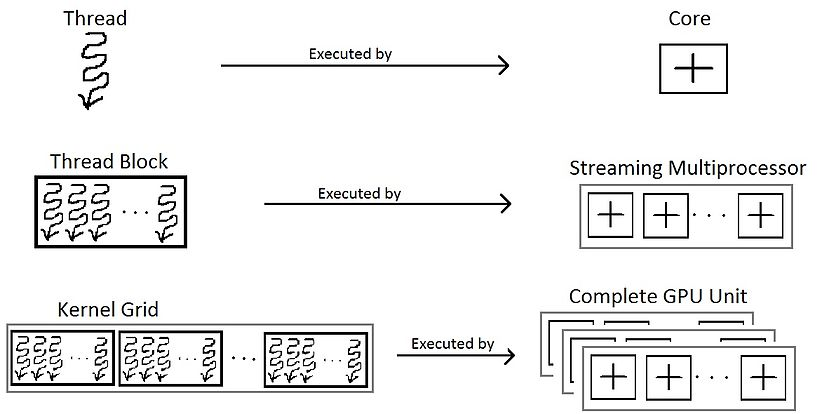
\includegraphics[width=0.8\textwidth]{cuda_kernel.jpg}
	\caption{CuDA thread block}
	\end{center}
\end{figure}

\begin{figure}[H]
	\begin{center}
		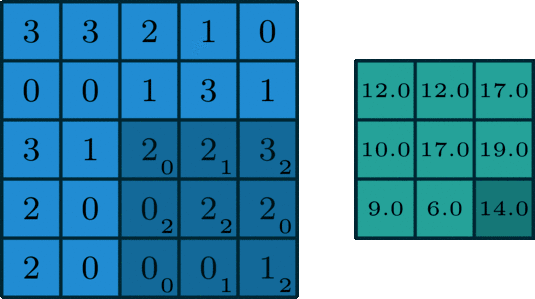
\includegraphics[width=0.5\textwidth]{convolutional_operation-8.png}
	\caption{Convolution operation}
	\end{center}
\end{figure}

\begin{figure}[H]
	\begin{center}
		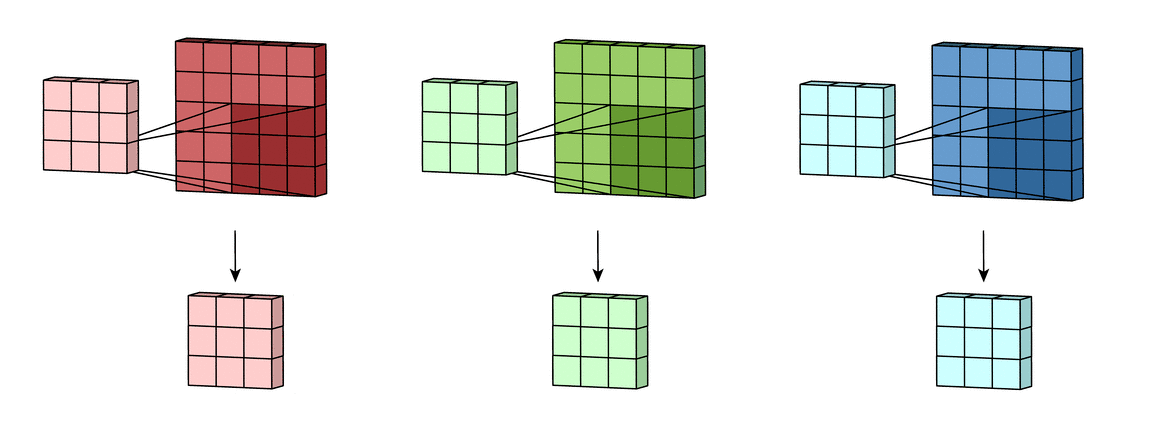
\includegraphics[width=\textwidth]{per_channel-9.png}
	\caption{Per-channel Convolution}
	\end{center}
\end{figure}

\subsection{Experimental setup}
\hspace{0.25 in}We implement the code in C .The code is compiled using NVCC. The object is run on an Nvidia GTX 1060 GPU with Pascal architecture having 6 Gigabytes of memory.

\newpage
\section{Results}
\hspace*{0.25 in}We run the algorithm on CPU as well as on GPU and we find that the algorithm runs exponentially faster when run on the GPU threads. 
The output is shown below:
\begin{figure}[H]
	\begin{center}
		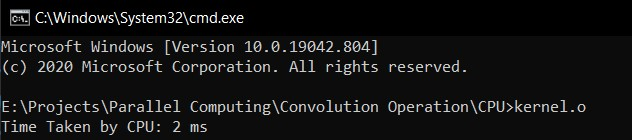
\includegraphics[width=\textwidth]{result_cpu.jpg}
	\caption{Time taken on CPU}
	\end{center}
\end{figure}
\begin{figure}[H]
	\begin{center}
		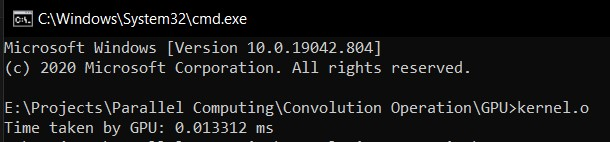
\includegraphics[width=\textwidth]{result_gpu.jpg}
	\caption{Time taken on GPU}
	\end{center}
\end{figure}

\newpage

\section{Conclusion}
\hspace*{0.25 in}Thus we have successfully implemented convolution operation on two matrices using CuDA.
\end{document}
